\documentclass[11pt]{article} 
\usepackage[margin=1in]{geometry} 
\usepackage{color,xcolor}
\usepackage[dvipsnames]{xcolor}
\usepackage{amssymb, amscd, amsmath, amsthm, graphicx, latexsym,wrapfig,array,seqsplit,xfrac}
\usepackage{dsfont}

\usepackage[makeroom]{cancel}

\usepackage{hyperref,comment,subcaption,graphicx}
\usepackage{microtype,numprint}
\usepackage{siunitx}

\usepackage{blkarray,multirow,multicol,booktabs,nicematrix,varwidth,paracol,hhline}

\usepackage{listings}

\usepackage{tikz,tkz-euclide,mathtools} 


\newtheorem*{ucorollary}{Corollary}
\newtheorem{theorem}{Theorem}[section]
\newtheorem{proposition}[theorem]{Proposition}
\newtheorem{lemma}[theorem]{Lemma}
\newtheorem{diagram}[theorem]{Figure}
\newtheorem{corollary}[theorem]{Corollary}

 
\newtheorem{definition}{Definition}[section]
\newtheorem{assumption}[theorem]{Assumption}
\newtheorem{conjecture}[theorem]{Conjecture}
\newtheorem{example}{Example}[section]
\newtheorem{remark}[theorem]{Remark}
\newtheorem{notation}[theorem]{Notation}
\newtheorem{refnumber}[theorem]{}

\newcommand{\N}{\mathbb{N}}
\newcommand{\Z}{\mathbb{Z}}
\newcommand{\F}{\mathbb{F}}
\newcommand{\R}{\mathbb{R}}
\newcommand{\C}{\mathbb{C}}
\newcommand{\Q}{\mathbb{Q}}
\newcommand{\bline}{\noindent\rule[0.5ex]{\linewidth}{1pt}}
\newcommand{\ndiv}{\nmid}
\newcommand{\nequiv}{\not\equiv}

\setcounter{MaxMatrixCols}{20}

\usepackage{blkarray, relsize}
\makeatletter
\newcommand{\setBAcolsep}[1]{\BA@colsep=#1}
\makeatother

\newcommand*\inb[1]{_{\textcolor{red}{#1}}}
\newcommand{\padic}{$p$-adic }
\newcommand{\bpadic}{p-adic }
\newcommand{\padics}{$p$-adics }


\usetikzlibrary{intersections,calc,angles}
\setlength{\tabcolsep}{0pt}
\NiceMatrixOptions{cell-space-limits = 1pt}


\newenvironment{myproof}[1][\proofname]{%
  \begin{proof}[#1]$ $\par\nobreak\ignorespaces
}{%
  \end{proof}
}

\newenvironment{problem}[2][Problem]{\begin{trivlist}
\item[\hskip \labelsep {\bfseries #1}\hskip \labelsep {\bfseries #2.}]}{\end{trivlist}}

\newenvironment{myproblem}[1][Problem]{\begin{trivlist}
    \item[\hskip \labelsep {\bfseries #1.}]}{\end{trivlist}}

\newenvironment{solution}
  {\renewcommand\qedsymbol{$~$}\begin{proof}[Solution]$ $\par\nobreak\ignorespaces}
  {\end{proof}}


\begin{document}

\title{An Introduction to $p$-adic Numbers}
\author{Rebekah Mayne\\
  Math 370, Fall 2024}
\date{}
\maketitle

\section{Background}
Kurt Hensel (1861-1941) introduced the idea of \padic numbers to mathematics in 1897, but had been working on them since 1893. His motivation was to ``transfer the power of calculus of series expansion from complex analysis to number theory.'' \cite{genesis}

\padic numbers were not necessarily popular at their start, however, they have gained notoriety, and specifically the Hasse-Minkowski Theorem was the crucial example of the application of \padic methods being the key to a problem. This is where the idea of checking a property ``everywhere locally'' became a central idea in number theory. \cite{Hist-talk} \padic numbers and \padic analysis has become an important idea in number theory as it gives a clearer way to understand and communicate congruences between integers, and allows for the use of methods from calculus and analysis to apply to number theory problems. While there are a few ways to approach \padic numbers, notably the way that Hensel was trying to extend an analogy between $\Z$ and it's field of fractions $\Q$, and the ring $\C[X]$ of polynomials with complex coefficients, together with its field of fractions $\C(X)$ that is discussed later, but first I will approach it in a somewhat more approachable way.



\section{Overview of \padic Numbers}
\padic numbers are alternatives way of organizing the rationals and filling in the gaps between them, similar to how the irrational numbers act in this regard.

The general idea surrounding the representation of \padic numbers is that they measure the frequency that each power of a prime $p$ appear in the base $p$ expansion of a number. \padic numbers are generally written the same as a base $p$ representation of the numbers. We will use the notation that $a\inb{p}=x$ means that $a$ is the base $p$ representation of $x$. So for example, the way that we would write 35 in base 3, is as follows,
\[
  35 = 1 \times 3^3 + 0 \times 3^2 + 2 \times 3^1 + 1 \times 3^0 = 1021 \inb{3}
\]
This gives rise to our following definitions
\begin{definition}
  For any rational number $x$ and any positive prime $p$ we can create the \textbf{p-adic expansion of x} as
  \begin{align*}
    x & = a_{n_0}p^{n_0} + a_{n_0+1}p^{n_0+1} + \cdots \\
    x & = \sum_{i\geq n_0} a_i p^i
  \end{align*}
  Remember that if $x$ is a positive integer, then it is simply its expansion in base $p$.

  Let's use the notation that $a\inb{p}$ means that $a$ is a \padic expansion of something that expands to $a$.
\end{definition}

Let's work out some simple examples to understand how this works practically.

We can see that $155=1\cdot 5^3+ 1 \cdot 5^2 + 1 \cdot 5 + 0$, so $155=1110_5$, then we want to show the notation that
\[
  \frac{155}{25} = \frac{1\cdot 5^3+ 1 \cdot 5^2 + 1 \cdot 5 + 0}{5^2} = 1\cdot 5^1+ 1 \cdot 5^0 + 1 \cdot 5^{-1} + 0^{-2} = 11.10\inb{5}
\]

Also see that $101=4\cdot 5^2 +0 \cdot 5+ 1$, so $101=401\inb{5}$, then we see that
\begin{align*}
  \begin{matrix}
    ~ & 155 & = & 1110\inb{5}           \\
    + & 101 & = & \phantom{1}401\inb{5} \\
    \hline
    ~ & 256 & = & 2011\inb{5}           \\
  \end{matrix}
\end{align*}
This is true since $265 =2\cdot 5^3 + 0\cdot 5^2 + 1 \cdot 5 + 1$. So we see that addition works in this system. Formally we can also see this,

\begin{proof}
  Let $x=a_0+a_1p+a_2p^2 +a_3p^3 + \cdots$ and $y=b_0+b_1p+b_2p^2 +b_3p^3 + \cdots$ where all $a_i,b_i\in \{1,2,\cdots, (p-1)\}$
  Then,
  \begin{align*}
    x + y & = (a_0+a_1p+a_2p^2 +a_3p^3 + \cdots)+ (b_0+b_1p+b_2p^2 +b_3p^3 + \cdots) \\
          & = (a_0+b_0)p^0 +(a_1+b_1)p+(a_2+b_2)p^2 +(a_3+b_3)p^3 + \cdots           \\
  \end{align*}
  If $a_i+b_i\leq p-1$ then there is no issue, if $a_i+b_i\geq p$ then we can separate sums of $p$ until it is less than $p$, let that be $n$ sums, so we can see within the sum that we have
  \begin{align*}
     & = \cdots + (a_i+b_i+np)p^i + (a_{i+1}+b_{i+1})p^{i+1} + \cdots         \\
     & = \cdots + (a_i+b_i)p^i + np^{i+1} + (a_{i+1}+b_{i+1})p^{i+1} + \cdots \\
     & = \cdots + (a_i+b_i)p^i + (a_{i+1}+b_{i+1}+n)p^{i+1} + \cdots          \\
  \end{align*}
  This will continue on for all $i$, until the right hand side is also a \padic expansion, so addition is possible in \padic expansion.
\end{proof}

We can also see that multiplication works by example, where we have $p=5$, $x=21$, $y=3$, we have that $21=41\inb{5}$ and $3=3\inb{5}$ let's see that
\[
  \begin{matrix}
    ~      & 4    & 1 & \inb{5} \\
    \times & ~    & 3 & \inb{5} \\
    \hline
    ~      & (12) & 3 & \inb{5} \\
  \end{matrix}
\]
We can't have 12, but we can see that $12=22\inb{5}$, so we have $41_5\cdot 3\inb{5} = 223\inb{5}$. We can check that $21\cdot3= 63$, and $63=2\cdots 5^2 + 2\cdot 5 + 3$, so $63=223\inb{5}$.




But, this is not a new system, the focus was on extending the analogy to the rational fractions.

To actually calculate fractions into a \padic representation, we can use long division methods to find the expansion for rational fractions. For example let's use $p=5$ and find $\frac{1}{11}$, we want to repeatedly find $r_i$ and $q_i$ so that $r_i+5q_i=q_{i-1}$ and we use that $x=q_0$, we also need all $r_i\in\{1,2,3,4\}$,
\begin{align*}
  \frac{1}{11}   & = 5 \cdot \frac{-2}{11} + 1 \\
  \intertext{We can see that we chose these because 1 is the only possible $r_1$ that results in a numerator divisible by 5}
  \frac{-2}{11}  & = 5 \cdot \frac{-7}{11} + 3 \\
  \frac{-7}{11}  & = 5\cdot \frac{-8}{11} + 3  \\
  \frac{-8}{11}  & = 5\cdot \frac{-6}{11} + 2  \\
  \frac{-6}{11}  & = 5\cdot \frac{-10}{11} + 4 \\
  \frac{-10}{11} & = 5\cdot \frac{-2}{11} + 0  \\
\end{align*}
We can see that once we hit $\sfrac{-2}{11}$, we have already found this, so our expansion is $\sfrac{1}{11}=\overline{04233}1\inb{5}$.


We can check this by doing the following: (reminder that 11 is $21\inb{5}$),

\[
  \begin{matrix}
    ~      & ~            & 0             & 4             & 2             & 3              & 3            & 1 & \inb{5} \\
    \times & ~            & ~             & ~             & ~             & ~              & 2            & 1 & \inb{5} \\
    \hline
    ~      & \cancel{3}^5 & \cancel{0}^2  & \cancel{4}^6  & \cancel{2}^4  & \cancel{3}^{4} & 3            & 1 & \inb{5} \\
    +      & 0            & 8             & 4             & 6             & 6              & 2            & 0 & \inb{5} \\
    \hline
    ~      & \cancel{5}^0 & \cancel{10}^0 & \cancel{10}^0 & \cancel{10}^0 & \cancel{10}^0  & \cancel{5}^0 & 1 & \inb{5} \\
  \end{matrix}
\]
We can see that this process continues to give us zeros infinitely to the left, so we can see that $\overline{04233}1\inb{5} \cdot 11=1$, or that $\overline{04233}1\inb{5}=\sfrac{1}{11}$.


The way that we think of 'size' in the \padic numbers is a little counterintuitive, as we want to think of our smallest numbers as the ones with the most factors of $p$. So we want to think of things like $162=3^4\cdot 2$ as smaller than something like $64=2^6$, since 162 has more factors of 3 than 64 does.




Another way to think about \padic numbers that is described in Houston-Edwards' article \cite{quant} is thinking of the modular 'rooms' and levels of powers of $p$, where two numbers are in a room if they are congruent mod $p$, and each level is a power of $p$.
\begin{figure}[h!]
  \centering
  \begin{subfigure}{0.29\textwidth}
    \centering
    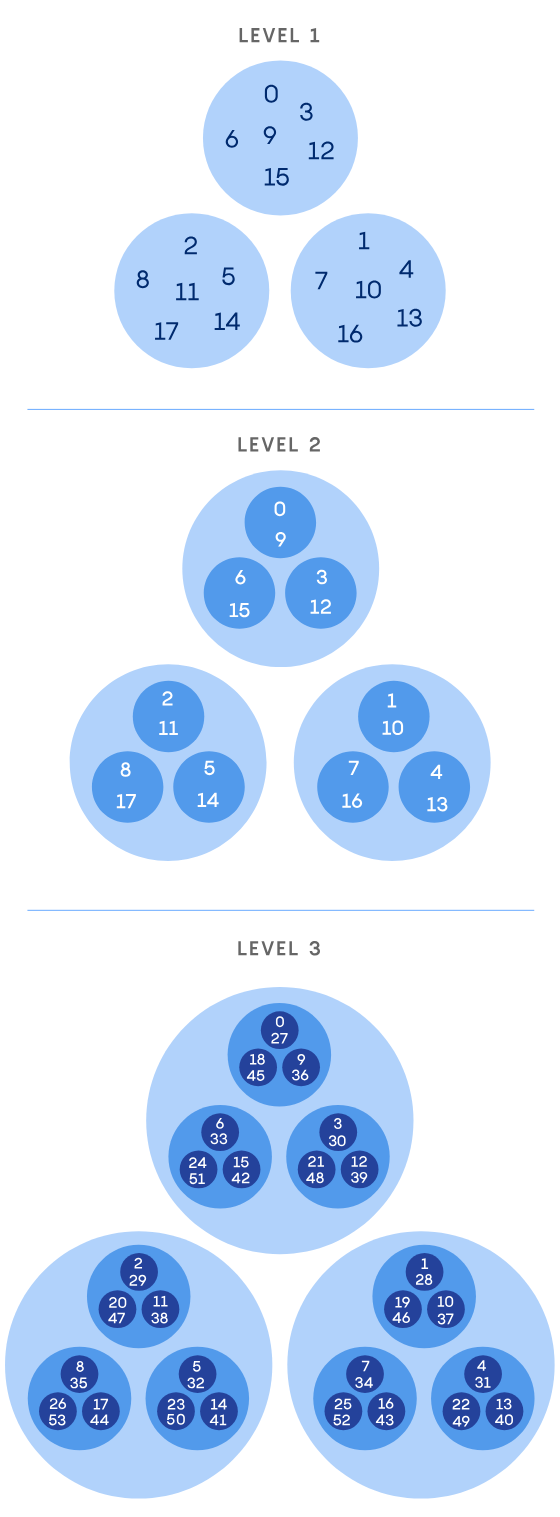
\includegraphics[height=.2\textheight,trim={2.5cm 30cm 2.5cm 1.2cm},clip]{levels.png}
    \caption{Level 1 (Mod 3).}
    \label{fig:first}
  \end{subfigure}
  \hfill
  \begin{subfigure}{0.30\textwidth}
    \centering
    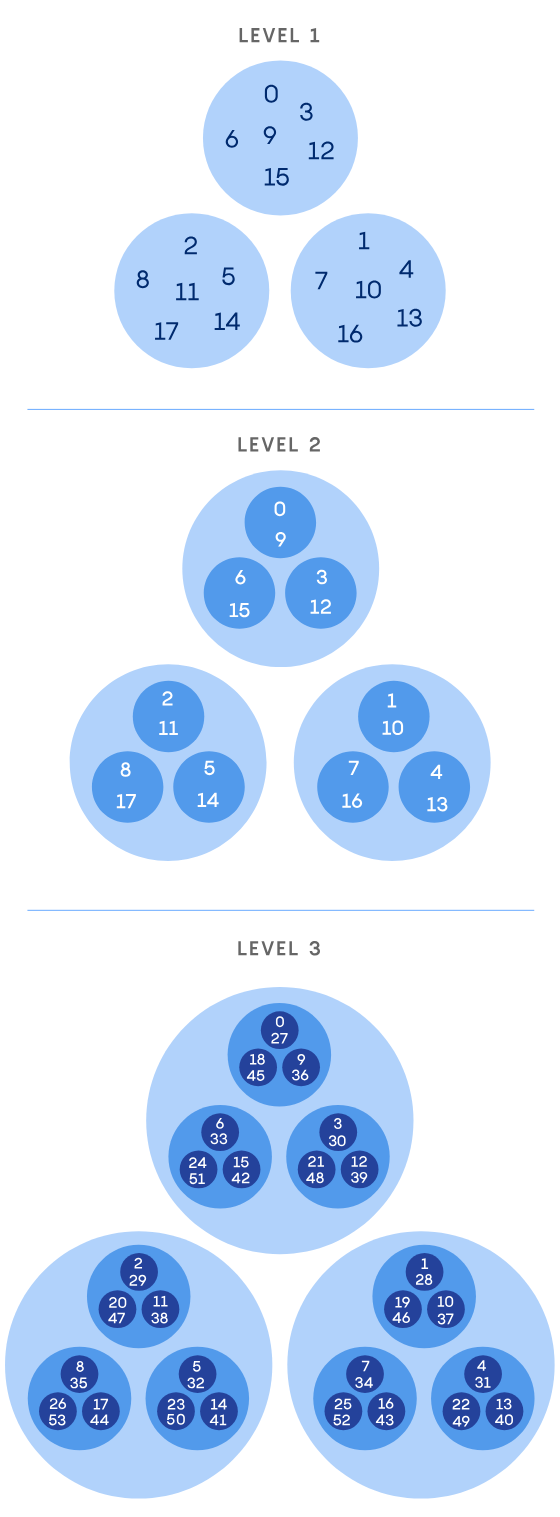
\includegraphics[height=.2\textheight,trim={1cm 17cm 1cm 12cm},clip]{levels.png}
    \caption{Level 2 (Mod 9).}
    \label{fig:second}
  \end{subfigure}
  \hfill
  \begin{subfigure}{0.30\textwidth}
    \centering
    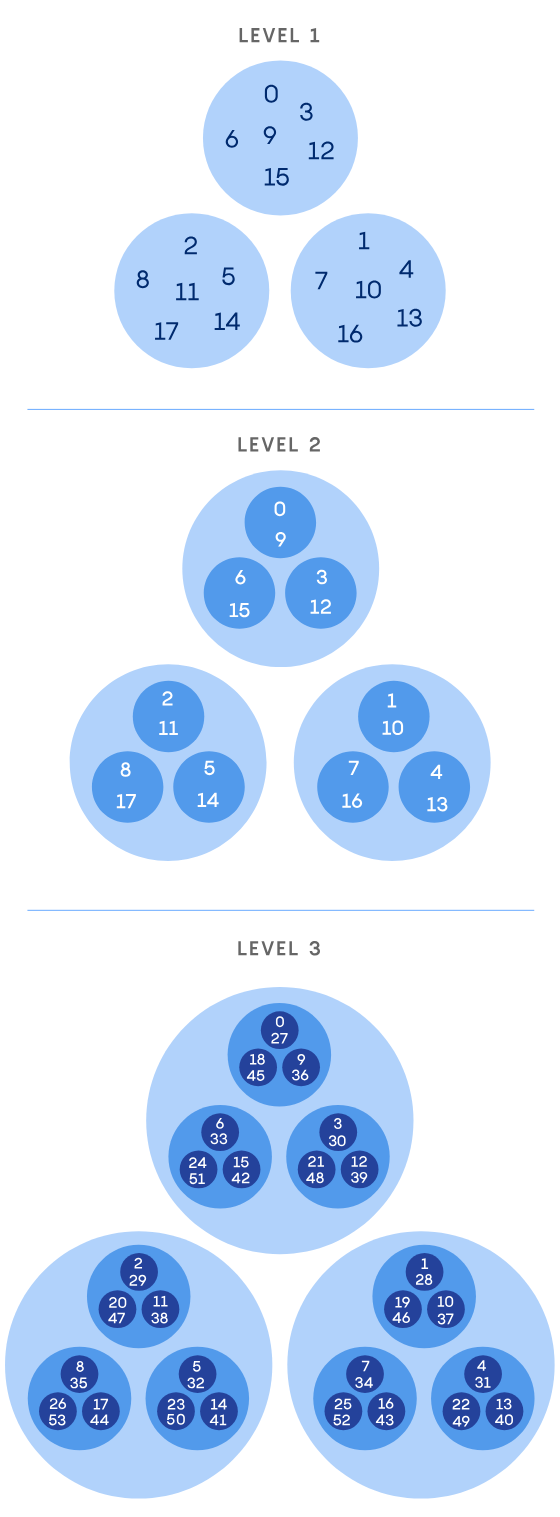
\includegraphics[height=.2\textheight,trim={0 0 0 25.5cm},clip]{levels.png}
    \caption{Level 3 (Mod 27).}
    \label{fig:third}
  \end{subfigure}

  \caption{\padic number 'rooms' visualization from \cite{quant}}
  \label{fig:figures}

\end{figure}

So thinking in 3-adic still, we have rooms in mod 3, so we start with our first level where we have rooms shown in light blue. Then level 2 we are in mod $3^2=9$, and we have the rooms within each level 1 room. Then level 3 are are in mod $3^3=27$, and we have the rooms within the rooms of level 2 within the rooms of level 1. This continues on infinitely with increasing powers of 3. This creates a way to intuitively feel what integers are closer to each other in the \padic numbers, as integers are closer together when they share a room at higher levels of the tower, and we remember that 0 will always be in the highest power of 3 room.

For our metaphor, expanding to the rational fractions means extending our tower into the basement. Numbers with larger powers of $p$ in the \textit{numerator} are smaller, and numbers with larger powers of $p$ in the \textit{denominator} are larger. So $\sfrac{1}{27}$ is larger than $\sfrac{81}{4}$ in 3-adics.





Let's next consider how to find a $-x$ in the \padics.
\begin{solution}
  To find $-x$ lets first consider a concrete case where we just try to find -1, let us look at the following for some prime $p$ in \padic numbers
  \[
    \begin{matrix}
      ~ & \cdots & \cancel{(p-1)}^{p} & \cancel{(p-1)}^{p} & \cancel{(p-1)}^{p} & \cancel{(p-1)}^{p} & (p-1) & \inb{p} \\
      + & \cdots & 0                  & 0                  & 0                  & 0                  & 1     & \inb{p} \\
      \hline
      ~ & \cdots & 0                  & 0                  & 0                  & 0                  & 0     & \inb{p} \\
    \end{matrix}
  \]
  So we can see that $-1=\cdots(p-1)(p-1)(p-1)\inb{p}$, and actually that $-a=\cdots(p-1)(p-1)(p-a)\inb{p}$ generally.
\end{solution}





Now we want to move on to defining some other means of evaluating in the \padics.


\begin{definition}\label{abs}
  Let $\mathds{k}$ be a field and let $\R^+ = {x \in \R : x \geq 0}$ be the set of all non-negative
  real numbers.
  An \textbf{absolute value} on $\mathds{k}$ is a function
  $$ |~| : \mathds{k} \rightarrow \R^+  $$
  that satisfies the following conditions:
  \renewcommand{\labelenumi}{\roman{enumi}) }
  \begin{enumerate}
    \item $|x|=0$ if and only if $x=0$;
    \item $|xy|=|x||y|$ for all $x,y\in \mathds{k}$;
    \item $|x+y|\leq |x|+|y|$ for all $x,y,\in \mathds{k}$.
  \end{enumerate}
  We say an absolute value on $\mathds{k}$ is \textbf{non-archimedean} if it satisfies the additional condition:
  \begin{enumerate}
    \item[iv) ] $|x+y|\leq \max\{|x|,|y|\}$ for all $x,y \in \mathds{k}$;
  \end{enumerate}
  otherwise, we will say that the absolute value is \textbf{archimedean}.
\end{definition}

Following this idea, we need to define two things specific to the \padic numbers.
We need to define the \padic valuation which can be thought of as the highest power of $p$ to divide a number, and can be formally defined by the following
\begin{definition}\label{valuation}
  Let $p\in\Z$ be any prime number. For any rational number $a$, where $a\neq 0$ we are able to write
  \[
    a = p^m \frac{u}{v} \; (m\in\Z, p\ndiv u,v)
  \]
  The \textbf{\bpadic valuation} of $a$ is $m$, we will denote it as $m = v_p(a)$. We will also set up that $v_p(0)=\infty$.
\end{definition}

Let's see what this actually looks like with some examples in base 3.
\begin{itemize}
  \item $v_3(35)$, we can see that $35=3^{0} \cdot 35$, so $v_3(35)=0$.
  \item $v_3(7776)$, we can see that $7776=3^5\cdot 32$, so $v_3(7776)=5$.
  \item $v_3(\sfrac{28}{27})$, we can see that $\sfrac{28}{27} = 3^{-3}\cdot 28$, so $v_3(\sfrac{28}{27})=-3$
\end{itemize}

For the following proofs in this section the following holds for all: Let $p=p_i$ for any $p_i\leq \max\{x,y\}$ and let $x=p_1^{e_1}p_2^{e_2}\cdots p_n^{e_n}$ and $y=p_1^{r_1}p_2^{r_2}\cdots p_n^{r_n}$ where $p_i$ is prime and for this case $e_i\geq 0$ and $r_i\geq 0$. (With the assertion that we will write $x$ and $y$ with every possible $p_i\leq \max\{x,y\}$).

\begin{lemma}\label{vprops}
  For all $x$ and $y$ $\in \Q$ we have
  \begin{itemize}
    \item [i)] $v_p(xy)=v_p(x)+v_p(y)$ and
    \item [ii)] $v_p(x+y)\geq \min\{v_p(x),v_p(y)\}$,
  \end{itemize}
\end{lemma}
\begin{proof}  On one side we have we have
  \begin{align*}
    v_{p_i}(xy) & = v_{p_i}(p_1^{e_1}p_2^{e_2}\cdots p_n^{e_n}\cdot p_1^{r_1}p_2^{r_2}\cdots p_n^{r_n}) \\
                & = v_{p_i}(p_1^{e_1+r_1}p_2^{e_2+r_2}\cdots p_n^{e_n+r_n})                             \\
                & = e_i+r_i                                                                             \\
  \end{align*}
  Then on the other side we have
  \begin{align*}
    v_{p_i}(x)+v_{p_i}(y) & = v_{p_i}(p_1^{e_1}p_2^{e_2}\cdots p_n^{e_n}) + v_{p_i}(p_1^{r_1}p_2^{r_2}\cdots p_n^{r_n}) \\
                          & = e_i + r_i
  \end{align*}
  So we can see that $v_p(xy)=v_p(x)+v_p(y)$, proving part $i$.

  Then, let $u_i=\min\{e_i,r_i\}$, and we can see that
  \begin{align*}
    v_{p_i}(x+y) & = v_{p_i} (p_1^{e_1}p_2^{e_2}\cdots p_n^{e_n} + p_1^{r_1}p_2^{r_2}\cdots p_n^{r_n})                                                   \\
                 & = v_{p_i} (p_1^{u_1}(p_1^{e_1-u_1}+p_1^{r_1-u_1})p_2^{u_2}(p_2^{e_2-u_2}+p_1^{r_2-u_2})\cdots p_n^{u_n}(p_n^{e_n-u_n}+p_n^{r_n-u_n})) \\
    \intertext{We can see that for all $i$, at least one of $e_i-u_i$ and $r_i-u_i$ will be 0, so if we set $w_i$ to be $\max\{e_i-u_i,r_i-u_i\}$ we can get the following}
    v_{p_i}(x+y) & = v_{p_i} (p_1^{u_1}(p_1^{w_1}+1)p_2^{u_2}(p_2^{w_2}+1)\cdots p_n^{u_n}(p_n^{w_n}+1))                                                 \\
    \intertext{Then, we can see that this means that}
    v_{p_i}(x+y) & \geq u_i                                                                                                                              \\
                 & \geq  \min\{e_i,r_i\}                                                                                                                 \\
    v_{p_i}(x+y) & \geq  \min\{v_{p_i}(x),v_{p_i}(y)\}
  \end{align*}
  Which is simply part $ii$, so we are done.

\end{proof}

\begin{definition}\label{pabs}
  If $a$ is a rational number and $p$ is a prime, we define the \textbf{\bpadic absolute value} of $a$ as
  \[
    |a|_p = p^{-v_p(a)}
  \]
  Note that $|0|_p=0$ because $v_p(0)=\infty$.
\end{definition}

Let's look at some examples of what this actually looks like calculating.
\begin{itemize}
  \item $|35|_3$ we see that this equals $3^{-v_3(35)}$, which we already found, so $|35|_3=3^{-0}=1$
  \item $|7776|_3$ we see that this equals $3^{-v_3(7776)}$, which we already found, so $|35|_3=3^{-5}=\sfrac{1}{3^5}=0.0041152263$
  \item $|\sfrac{28}{27}|_3$, we can see that this equals $3^{-v_3(\sfrac{28}{27})}$, which we already found, so $|\sfrac{28}{27}|_3=3^{3}=27$
\end{itemize}
We can see that this means that 7776 is smaller than 35 in 3-adic since it is closer to 0, and $\sfrac{28}{27}$ is larger than both, since it has negative factors of 3.


\begin{theorem}\label{p-non-arch}
  The \padic absolute value is non-archimedean.
\end{theorem}

\begin{proof}
  Using Lemma \ref{vprops} and Definition \ref{pabs} we have
  \begin{align*}
    |x+y|_{p_i} & = p_i^{-v_{p_i}(x+y)}                             \\
                & \leq \max\{p_i^{-v_{p_i}(x)}, p_i^{-v_{p_i}(y)}\} \\
    |x+y|_{p_i} & \leq \max\{|x|_{p_i}, |y|_{p_i}\}
  \end{align*}
  This is the definition of being non-archimedean.
\end{proof}



\section{Hensel's Origin of \padic Numbers}

Hensel's starting point for \padic numbers was an analogy between $\Z$ and it's field of fractions $\Q$, and the ring $\C[X]$ of polynomials with complex coefficients, together with its field of fractions $\C(X)$. The elements of these that will be used are defined as follows.
\begin{definition}
  An element of $f(X) \in \C(X)$ is a \textbf{rational function}, i.e., a quotient of two polynomials:
  \[
    f(X)= \frac{P(X)}{Q(X)}
  \]
  with $P(X)$,$ Q(X) \in \C[X]$, $Q(X) \neq 0$, we require $Q(X)$ to be monic (i.e. it's leading coefficient is 1)
\end{definition}
\begin{definition}
  An element $x\in \Q$ is a \textbf{rational fraction}, i.e. a quotient of two integers:
  \[
    x=\frac{a}{b}
  \]
  with $a,b\in \Z$, $b \neq 0$, we require $b>0$.
\end{definition}
The property of both rings $Z$ and $\C[X]$ that we need is that both have \textbf{unique factorization}.
In $\C[X]$ this means that any polynomial $P(X)$ can be expressed uniquely as
\[
  P (X) = a(X - \alpha_1)(X - \alpha_2)\cdots (X - \alpha_n),
\]
where $a$ and $\alpha_1,\alpha_2, \cdots, \alpha_n$ are complex numbers.

In $\Z$, this means any integer $x$ can be expressed uniquely as
\[
  \pm p_1^{e_1} \cdot p_2^{e_2} \cdots p_n^{e_n}
\]
where $p_i$ are unique primes and $e_i>0$ for all $i$.

What follows is the primary focus of the analogy that Hensel focused on: \textit{The primes $p \in \Z$ are analogous to the linear polynomials $X - \alpha \in \C[X]$.} Following this in the analogy is the analogy between algebraic numbers and algebraic functions where
\begin{definition}
  Given a polynomial with coefficients in $Z$, any root is an \textbf{algebraic number}; if a function is a root of a polynomial with coefficients in $\C[X]$, it is an \textbf{algebraic function}.
\end{definition}
Hensel's focus was on extending the analogy to expanding algebraic numbers in a similar way to expanding algebraic functions into power series as follows:
Suppose we are given a polynomial $P(X) \in \C[X]$ and a particular $\alpha \in \C$. Then we can write using Taylor expansion
\begin{align*}
  P(X) & = a_0 +a_1(X-\alpha)+a_2(X-\alpha)^2 +\cdots+a_n(X-\alpha)^n \\
       & = \sum_{i=0}^n a_i(X-\alpha)^i
\end{align*}
with $a_i\in \C$.
We can see that $(X-\alpha)$ is a prime in $\C[X]$, so for an extension to $\Z$ we would also want to use primes, so we will expand in a base $p$, so given a positive integer $x$ it would be
\begin{align*}
  x & = a_0 +a_1p+a_2p^2 +\cdots+a_np^n \\
    & = \sum_{i=0}^n a_ip^i
\end{align*}
with $a_i \in\Z$ and $0\leq a_i \leq p-1$.

We know that the expansion of algebraic functions gives us information that is local to powers of $X-\alpha$ and similarly, the expansion of algebraic numbers gives us the information that is local to powers of $p$.

Then we want to look at this in $\C(X)$, we know that given $f(X) \in \C(X)$ and $\alpha \in\C$, there is always an expansion
\begin{align*}
  f(X) = \frac{P(X)}{Q(X)} & = a_{n_0} +a_1(X-\alpha)^{n_0}+a_{n_0+1}(X-\alpha)^{n_0+1} +\cdots \\
                           & = \sum_{i\geq n_0} a_i(X-\alpha)^i
\end{align*}
This is the \textbf{Laurent expansion} in complex analysis, and can be obtained either through long division of the expansions of $P(X)$ and $Q(X)$ or by division with remainders.

There are a few reasons why this is more complicated, such as we can have $n_0<0$, meaning it can start with a negative exponent, which would mean that $\alpha$ is a root of $Q(X)$ and not of $P(X)$. This can be fixed by multiplying by $(X-\alpha)^{|n_0|}$, expanding the result into powers of $(x-\alpha)$ and thn diving again at the end. We also know the expansion will not usually be finite. It will only be finite when $Q(X)$ is a power of $(X-\alpha)$ when $f(X)$ is in lowest terms, and $Q(X)$ is monic.

Hensel wanted to extend the analogy between $Z$ and $\C[X]$ to include this construction. In our analogy, choosing $\alpha$ is the same as choosing a prime $p$, so we want our expansion to reflect information about the behavior of any rational number, and we can use this to create our \padic expansion.

\bibliographystyle{plain}
\bibliography{biblio}


\end{document}